\chapter{Figures} \label{sec:appendixFigures}

% -------------------------------------------------------------------------
% ACQUIRING SOURCE
% -------------------------------------------------------------------------

\begin{figure}[!ht]
  \centering
  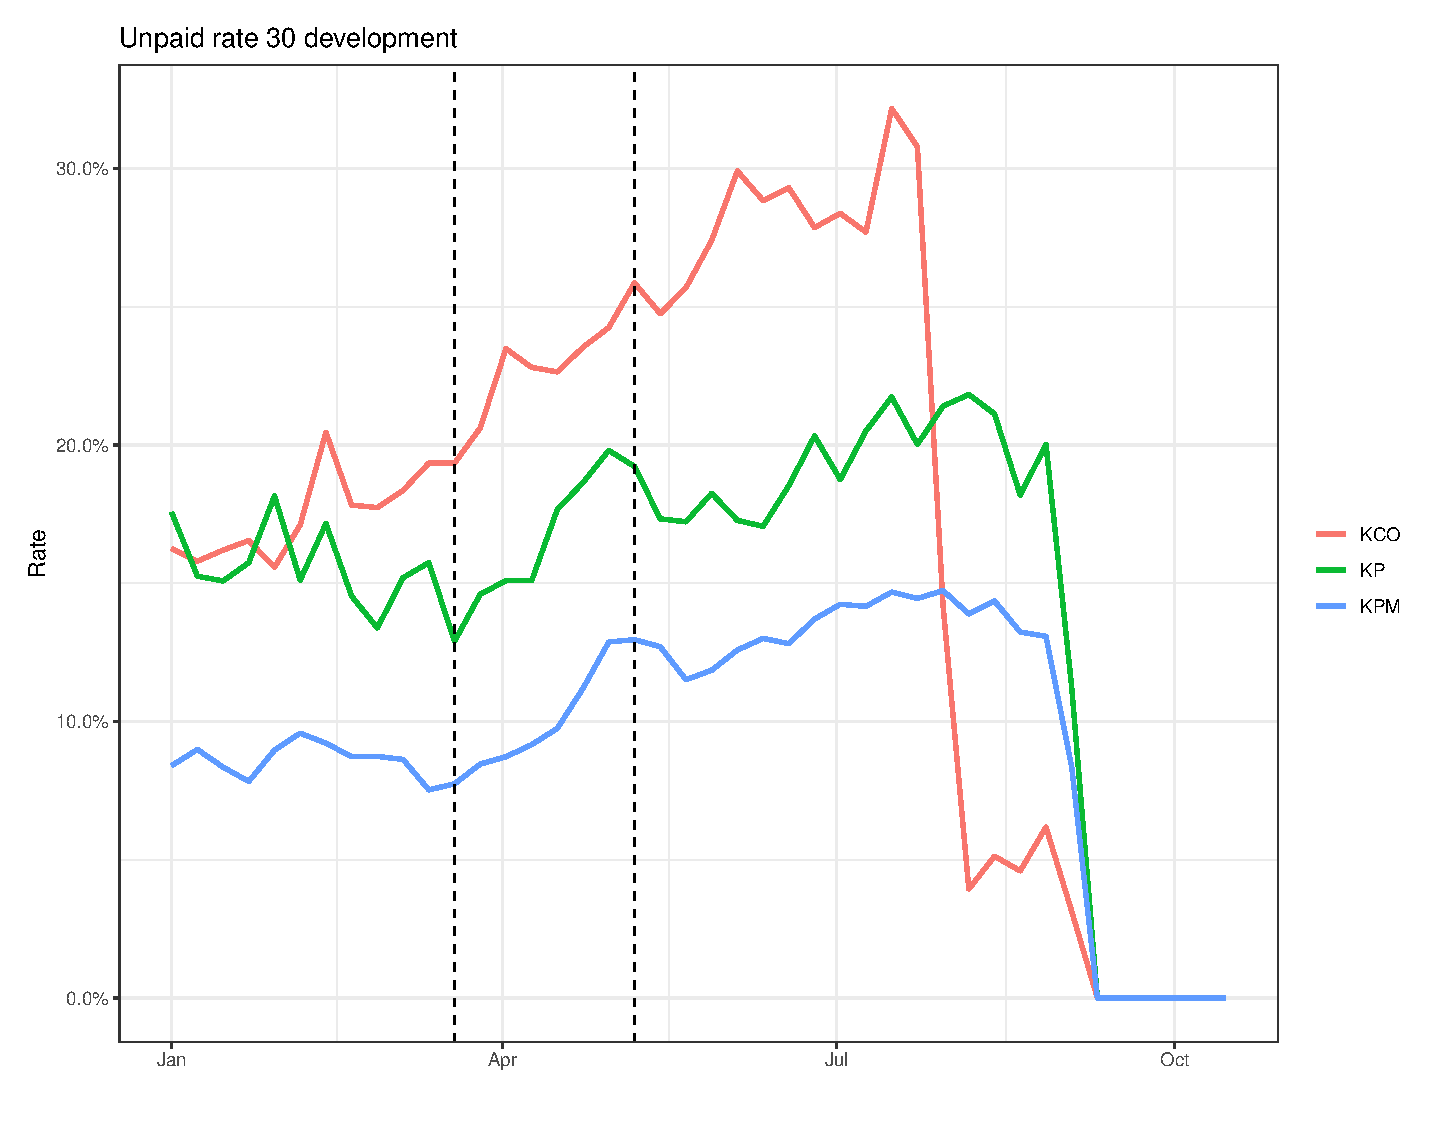
\includegraphics[width=5in,trim={0 0 0 0},clip]{content/figures/rate30_dev_nl_as.eps} 
  \caption{Unpaid rate 30 for the different acquiring sources. The increase is present within all acquiring sources but is more profound for KCO.}
  \label{fig:rate30_dev_as}
\end{figure}

\begin{figure}[!ht]
  \centering
  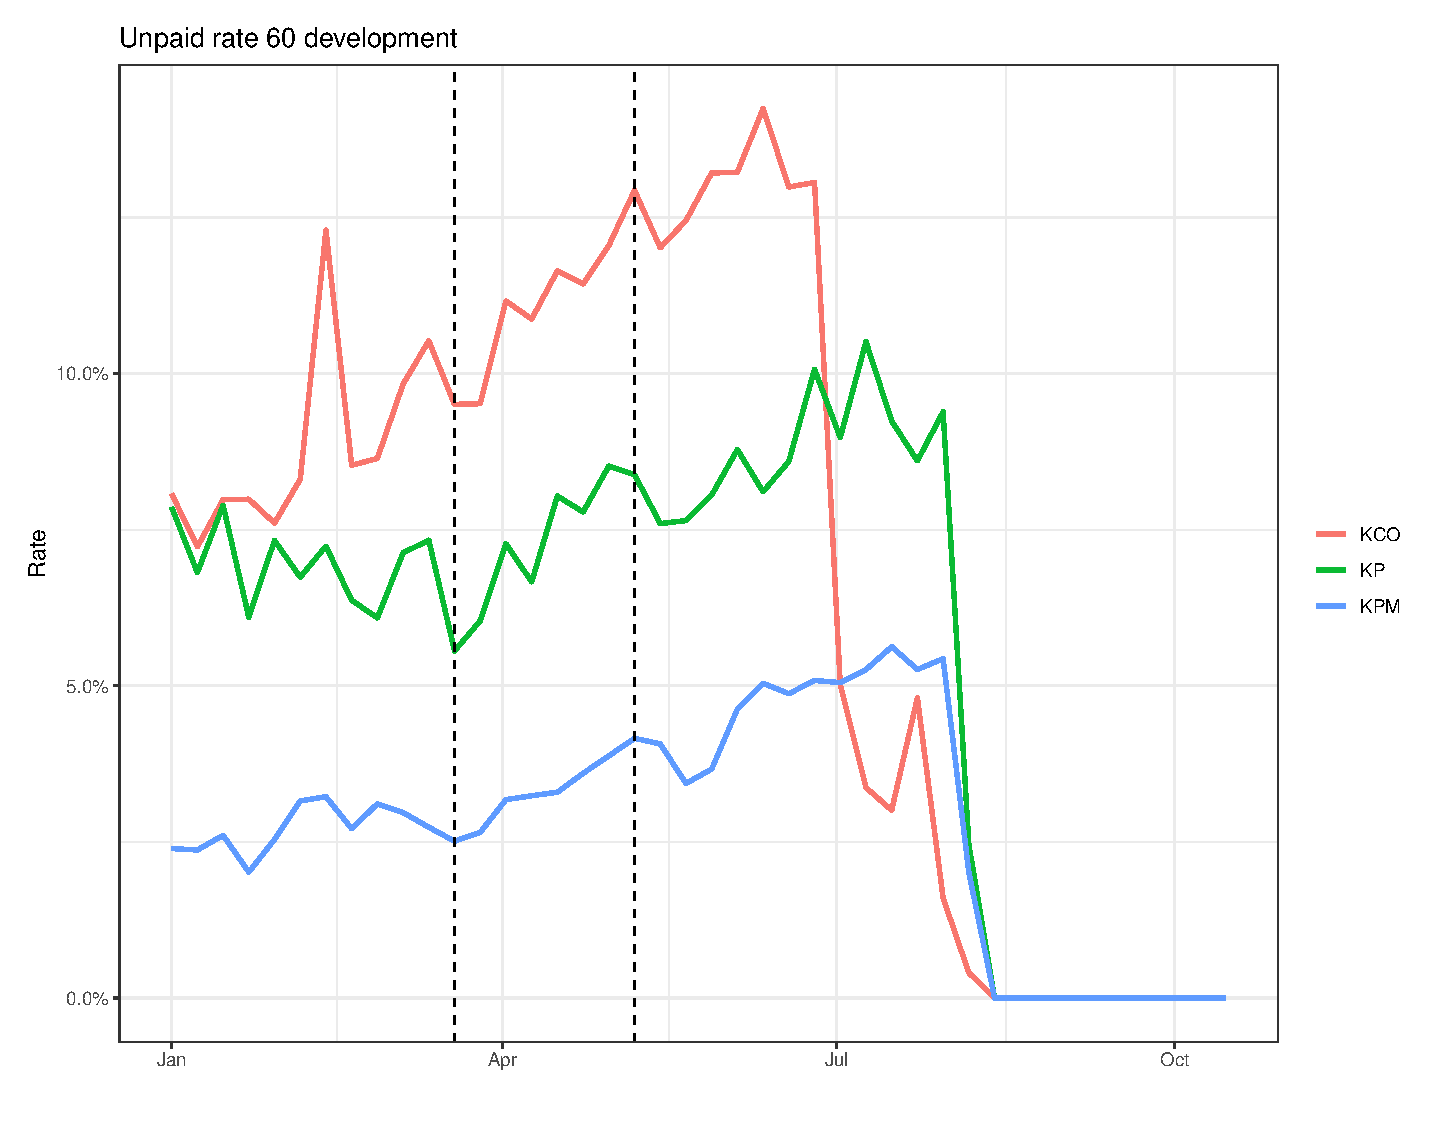
\includegraphics[width=5in,trim={0 0 0 0},clip]{content/figures/rate60_dev_nl_as.eps} 
  \caption{Unpaid rate 60 for the different acquiring sources. Same conclusions as for the unpaid rate 30 development.}
  \label{fig:rate60_dev_as}
\end{figure}

\begin{figure}[!ht]
  \centering
  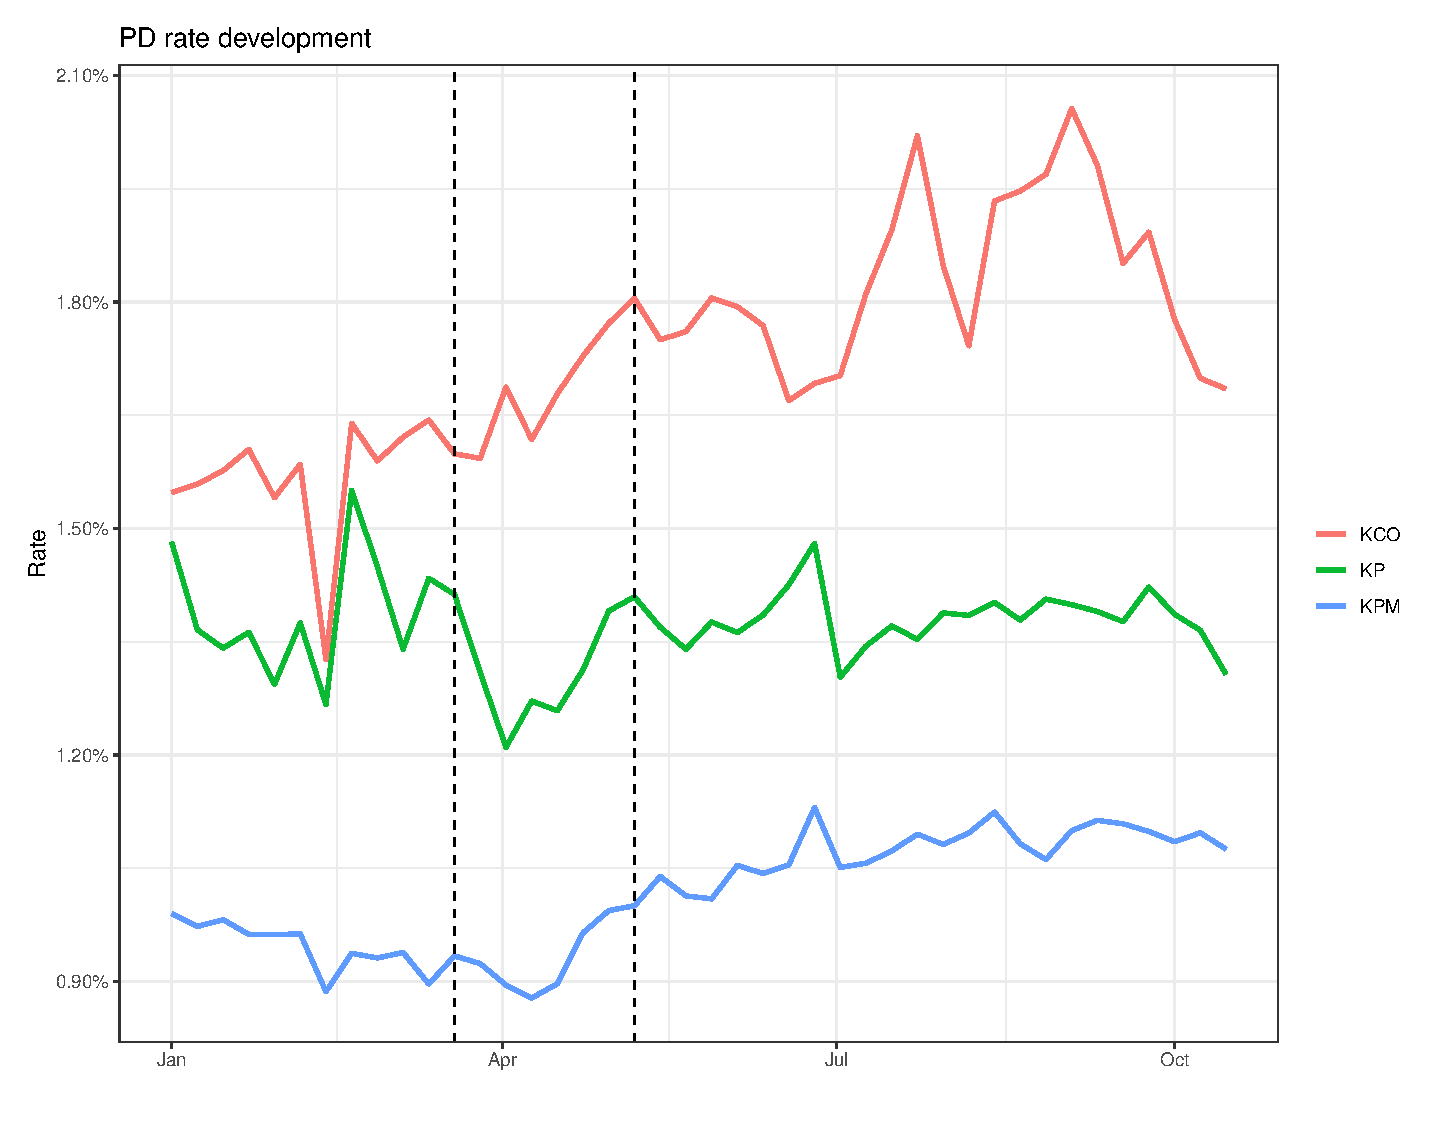
\includegraphics[width=5in,trim={0 0 0 0},clip]{content/figures/pd_dev_nl_as.eps} 
  \caption{PD development. The increase is mainly present for KCO and KPM. KP seems to have a stable PD rate but the volume for KP is quite small compared to KPM and KCO.}
  \label{fig:pd_dev_as}
\end{figure}

%\begin{figure}[!ht]
%  \centering
%  \includegraphics[width=5in,trim={0 0 0 0},clip]{content/figures/pd_dev_nl_as_ex_omoda.eps} 
%  \caption{PD development excluding Omoda. The increase in PD is still visible but the increase for KCO is much lower.}
%  \label{fig:pd_dev_as_ex_om}
%\end{figure}
%
%\begin{figure}[!ht]
%  \centering
%  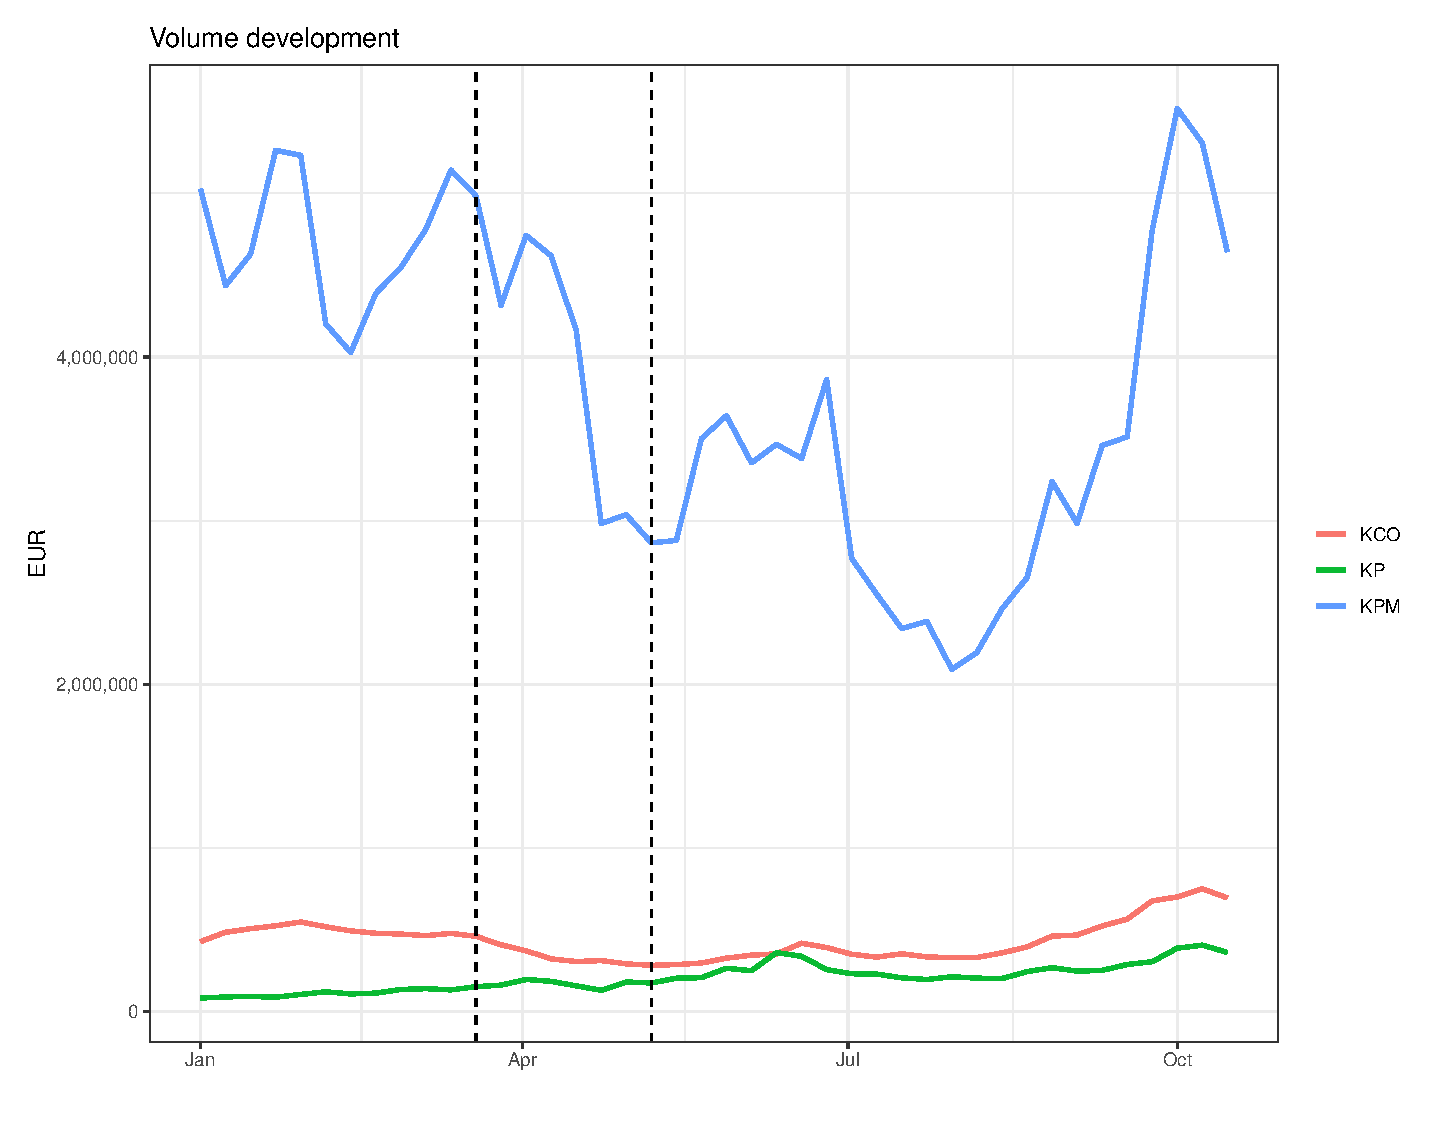
\includegraphics[width=5in,trim={0 0 0 0},clip]{content/figures/vol_dev_nl_as.eps} 
%  \caption{Volume development for the different acquiring sources. There seems to be a decline in KPM during the year. Sharp decline for KCO due to customer Omoda leaving KCO and entering KPM and KP.}
%  \label{fig:vol_dev_as}
%\end{figure}
%
%\begin{figure}[!ht]
%  \centering
%  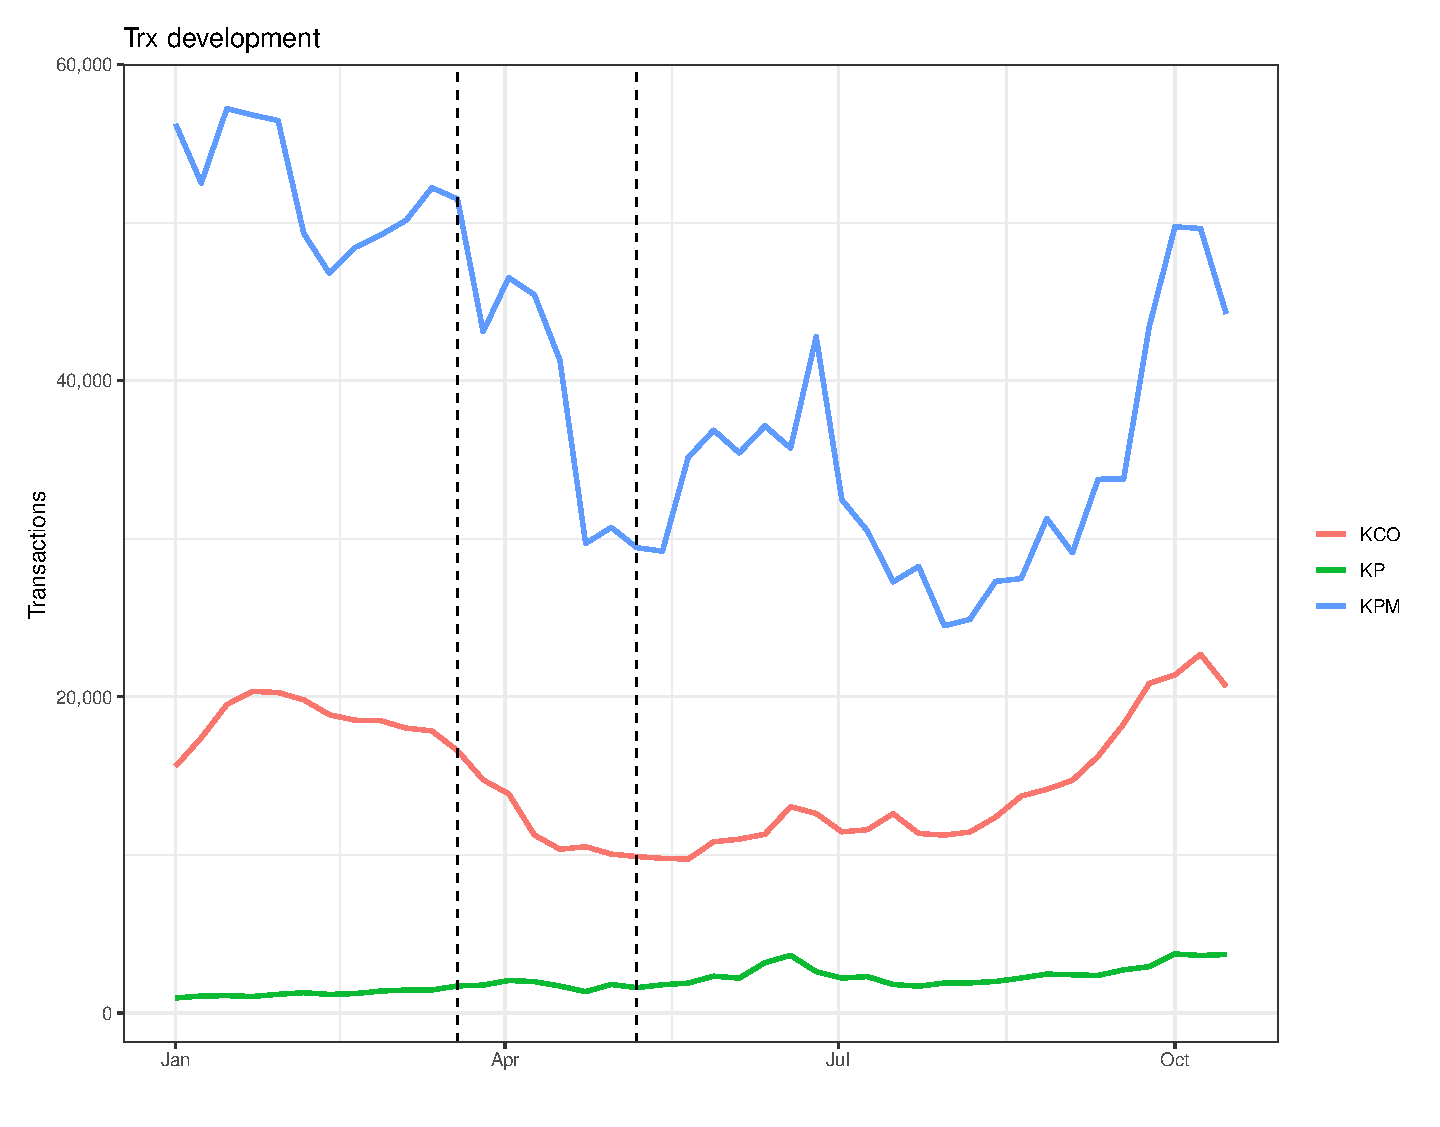
\includegraphics[width=5in,trim={0 0 0 0},clip]{content/figures/trx_dev_nl_as.eps} 
%  \caption{Transactions in NL. Follows volume development. The sharp decline in transactions for KCP is due to Omoda.}
%  \label{fig:trx_dev_as}
%\end{figure}
%
%\begin{figure}[!ht]
%  \centering
%  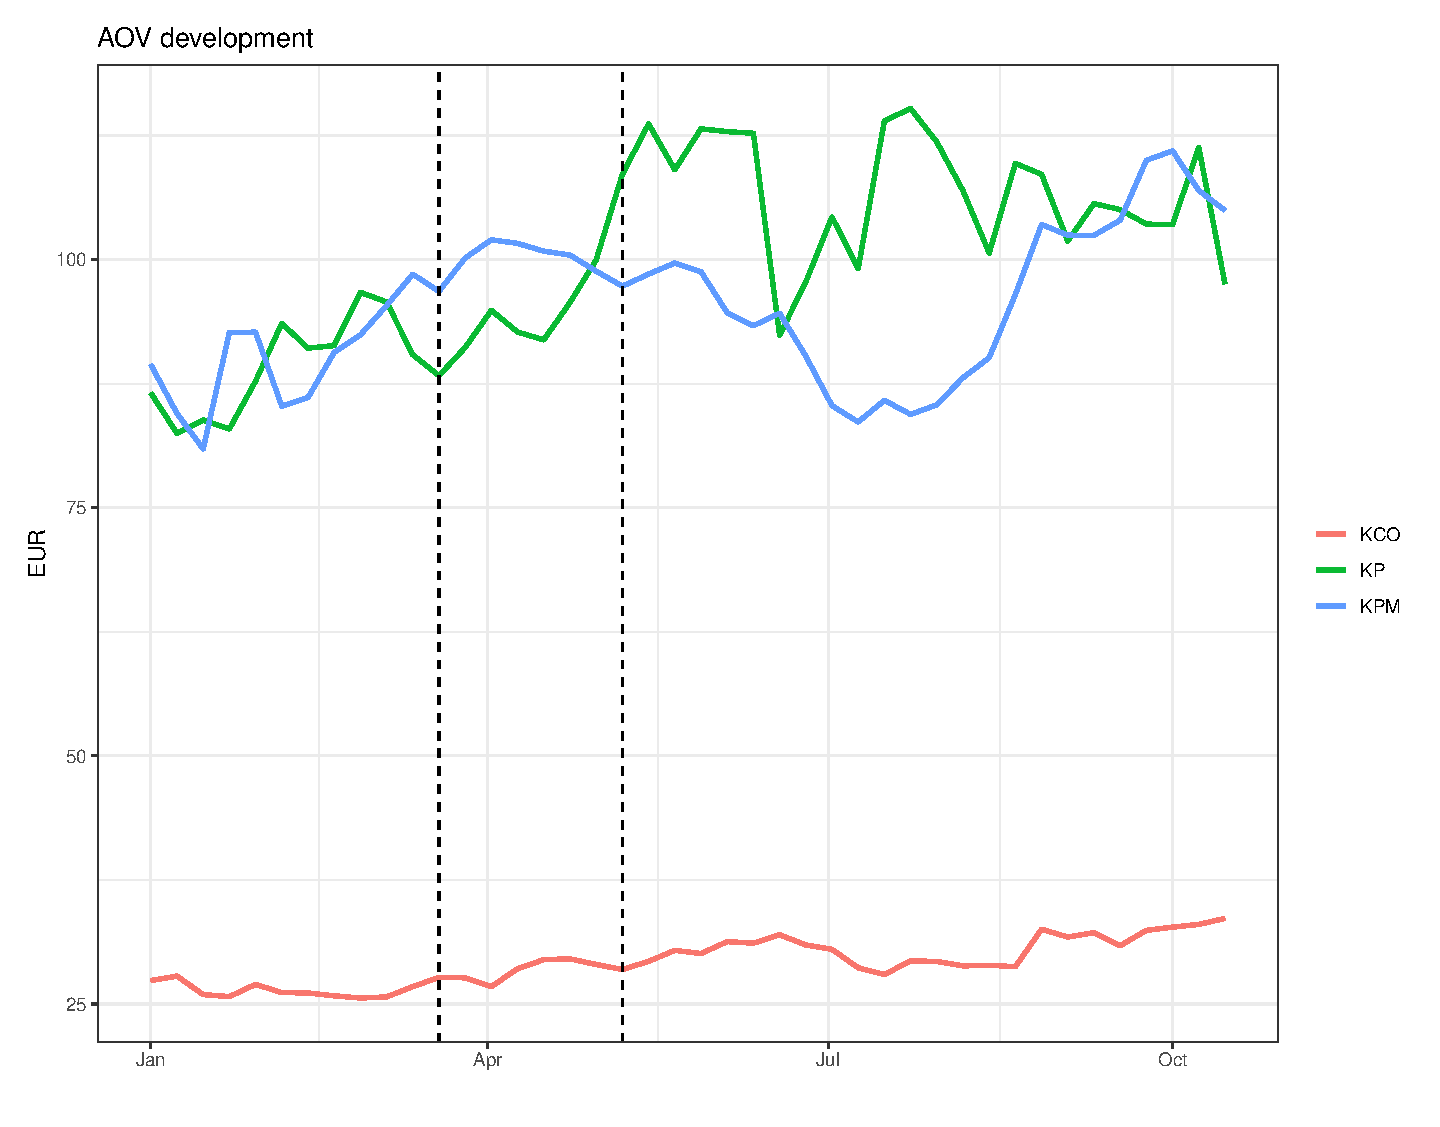
\includegraphics[width=5in,trim={0 0 0 0},clip]{content/figures/aov_dev_nl_as.eps} 
%  \caption{AOV development for the different acquiring sources. The AOV in KCO is largely influenced by Wish, which is why its on a much lower level than the other sources. Excluding Wish will higher the AOV to similar levels as the other sources. The decline in AOV is due to merchant Omoda.}
%  \label{fig:aov_dev_as}
%\end{figure}

% -------------------------------------------------------------------------
% MERCHANT SPECIFIC, ESTORE GROUP, ESTORE SEGMENT
% -------------------------------------------------------------------------

\begin{figure}[!ht]
  \centering
  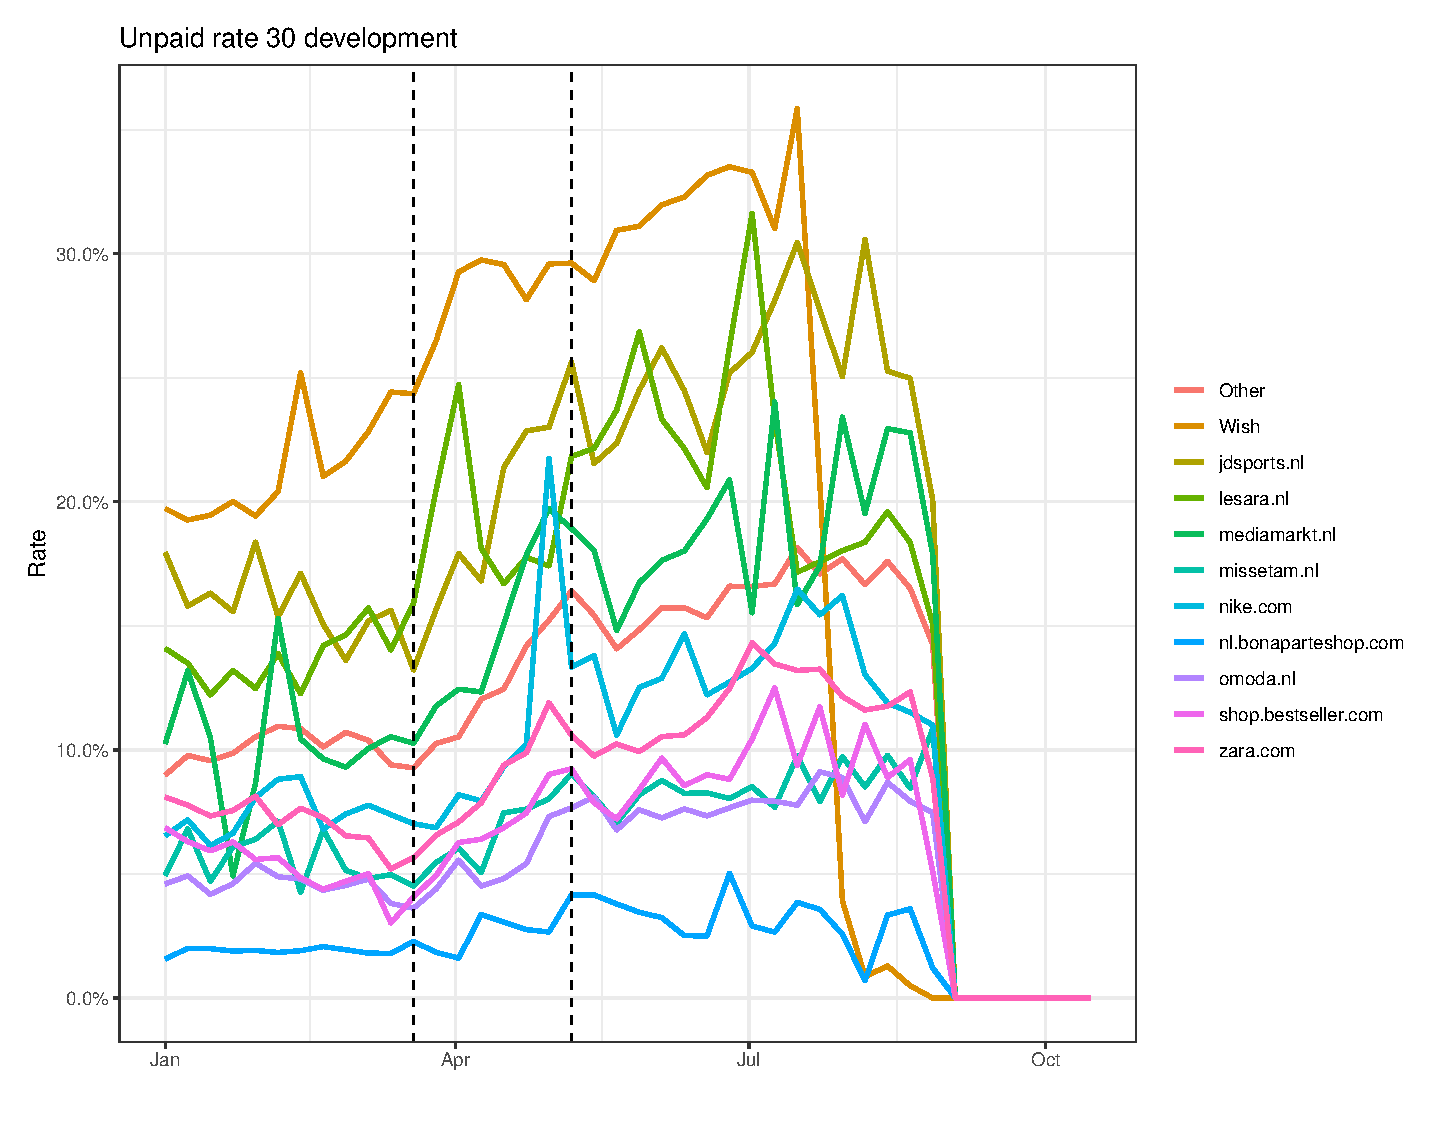
\includegraphics[width=5in,trim={0 0 0 0},clip]{content/figures/rate30_dev_nl_mer.eps} 
  \caption{Unpaid rate 30 for merchants. It is evident that the increase is present within more or less all merchants. Hence it is not possible to draw any conclusions about the increase just looking at specific merchants/groups/segments.}
  \label{fig:rate30_dev_mer}
\end{figure}

\begin{figure}[!ht]
  \centering
  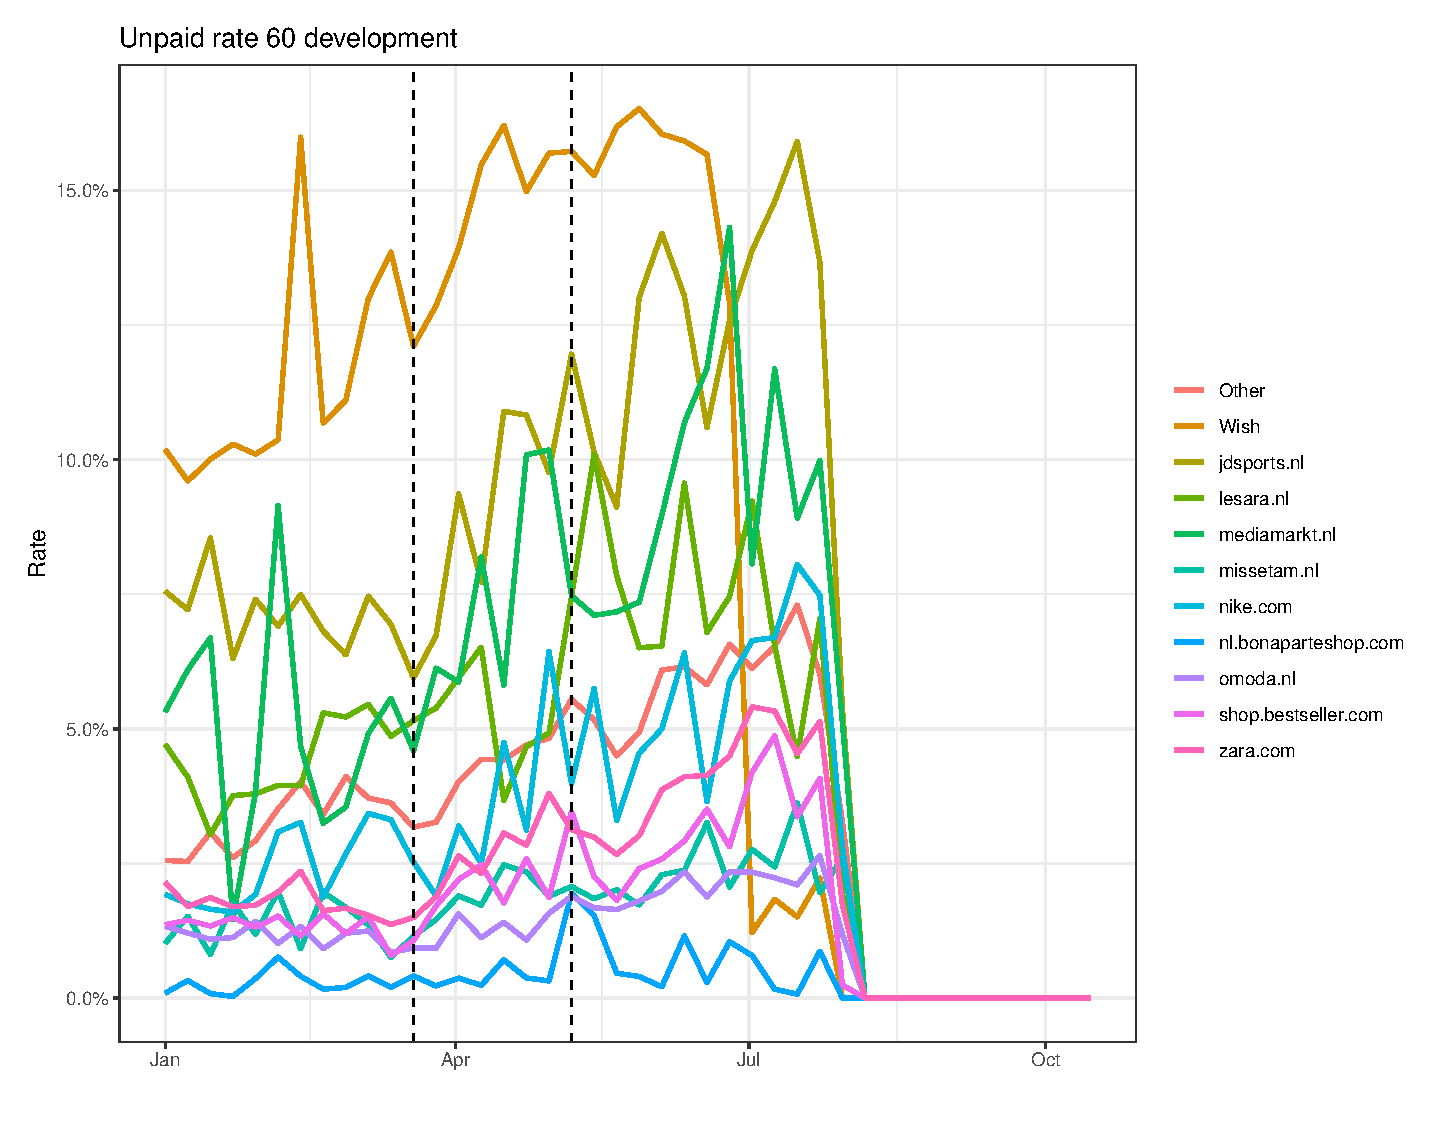
\includegraphics[width=5in,trim={0 0 0 0},clip]{content/figures/rate60_dev_nl_mer.eps} 
  \caption{Unpaid rate 60 for merchants. Similar development as for unpaid rates 30. Same reasoning. The increase is more present for some merchants than for others but on a whole the increase is within all merchants/groups/segments.}
  \label{fig:rate60_dev_mer}
\end{figure}

\begin{figure}[!ht]
  \centering
  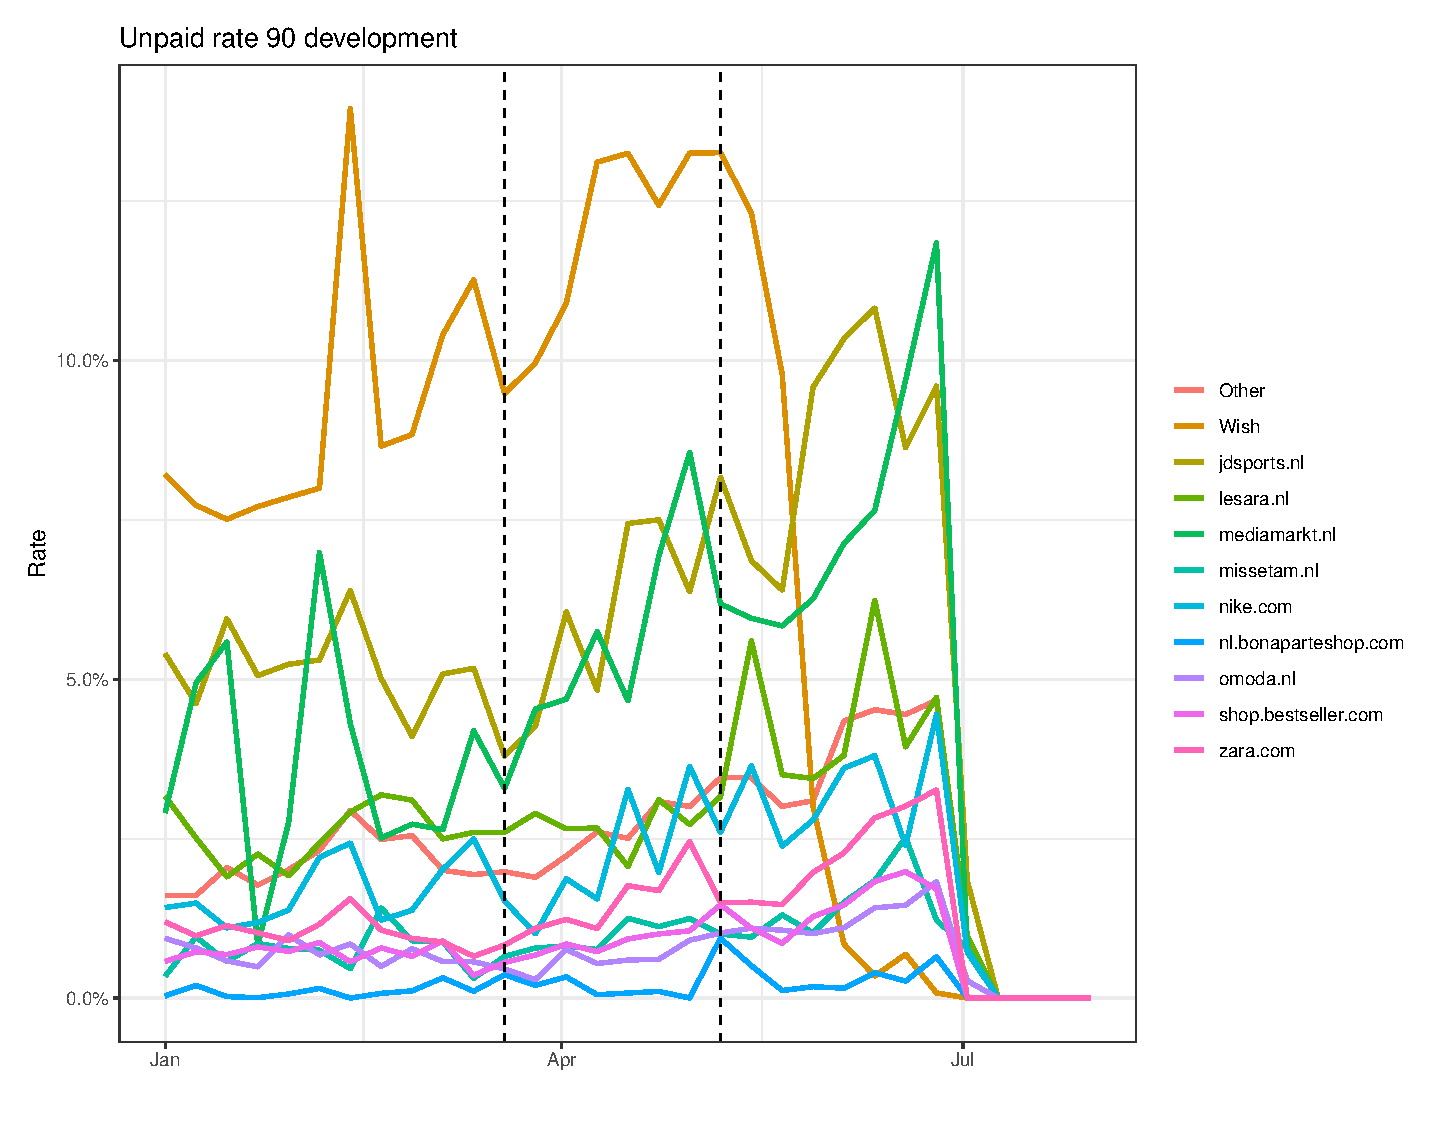
\includegraphics[width=5in,trim={0 0 0 0},clip]{content/figures/rate90_dev_nl_mer.eps} 
  \caption{Unpaid rate 90 for merchants. Similar development as for unpaid rates 30 and 60. Same reasoning. The increase is also here present within (more or less) all merchants/groups/segments.}
  \label{fig:rate90_dev_mer}
\end{figure}

\begin{figure}[!ht]
  \centering
  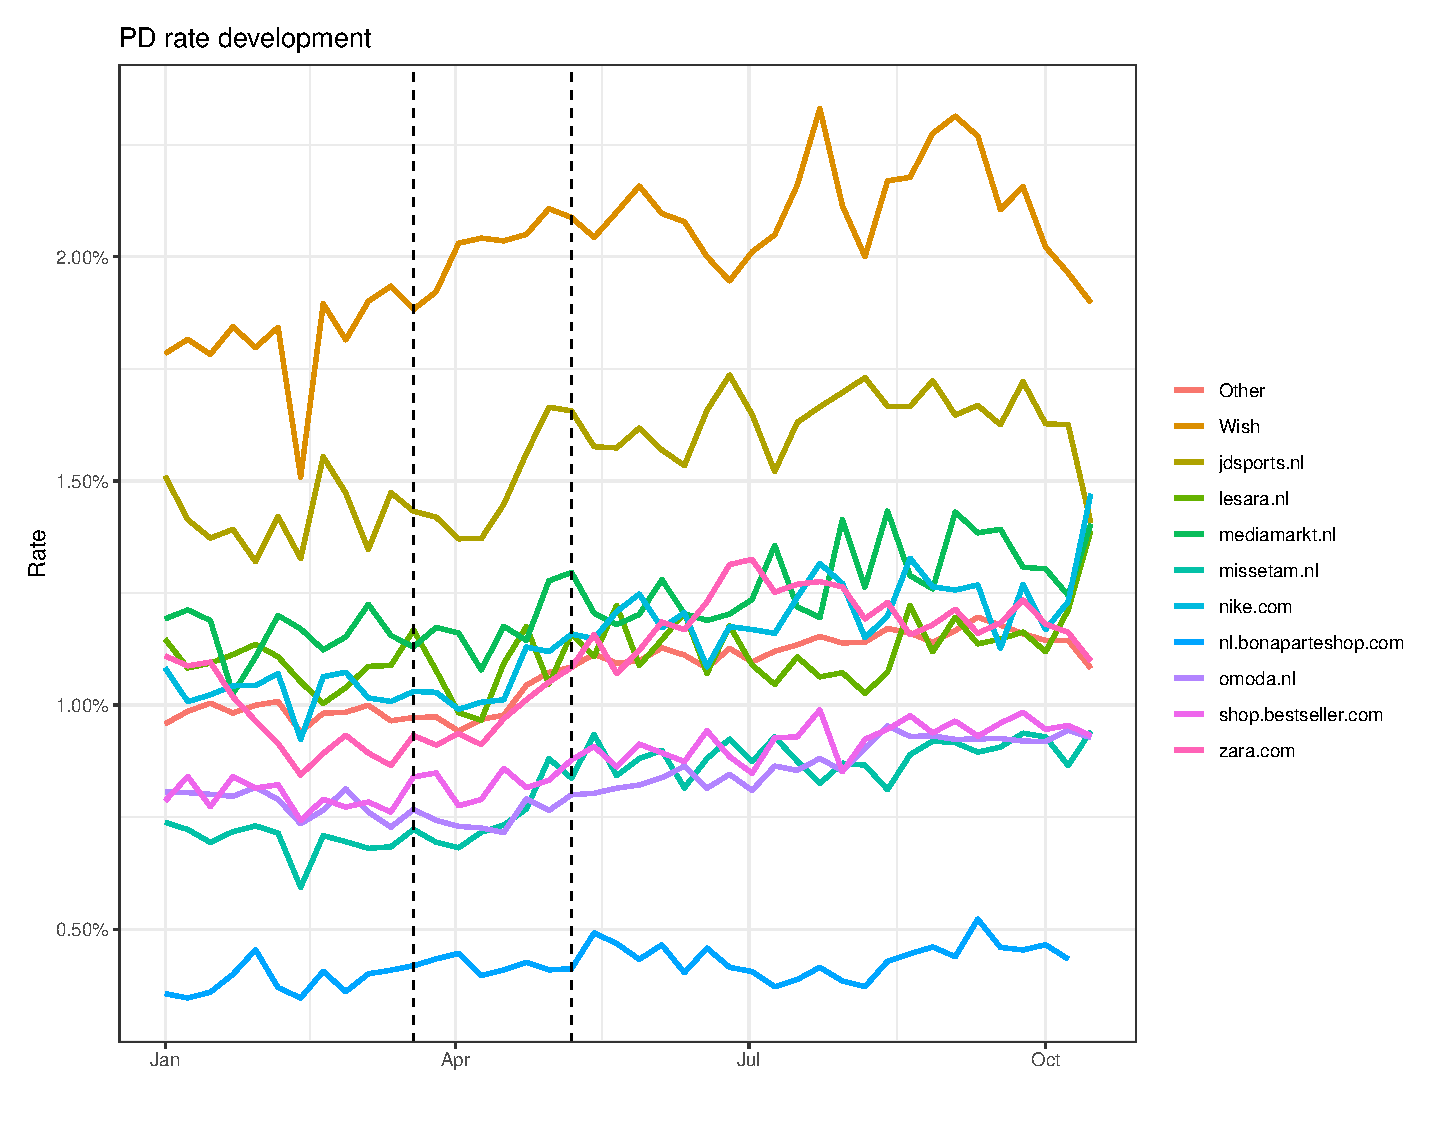
\includegraphics[width=5in,trim={0 0 0 0},clip]{content/figures/pd_dev_nl_mer.eps} 
  \caption{PD rate for merchants. Even though not at evident as for the other unpaid rates, the PD rates are increasing as well. This suggest that the population entering the market entail a higher risk than previous.}
  \label{fig:pd_dev_mer}
\end{figure}

% -------------------------------------------------------------------------
% SCORE
% -------------------------------------------------------------------------

\begin{figure}[!ht]
  \centering
  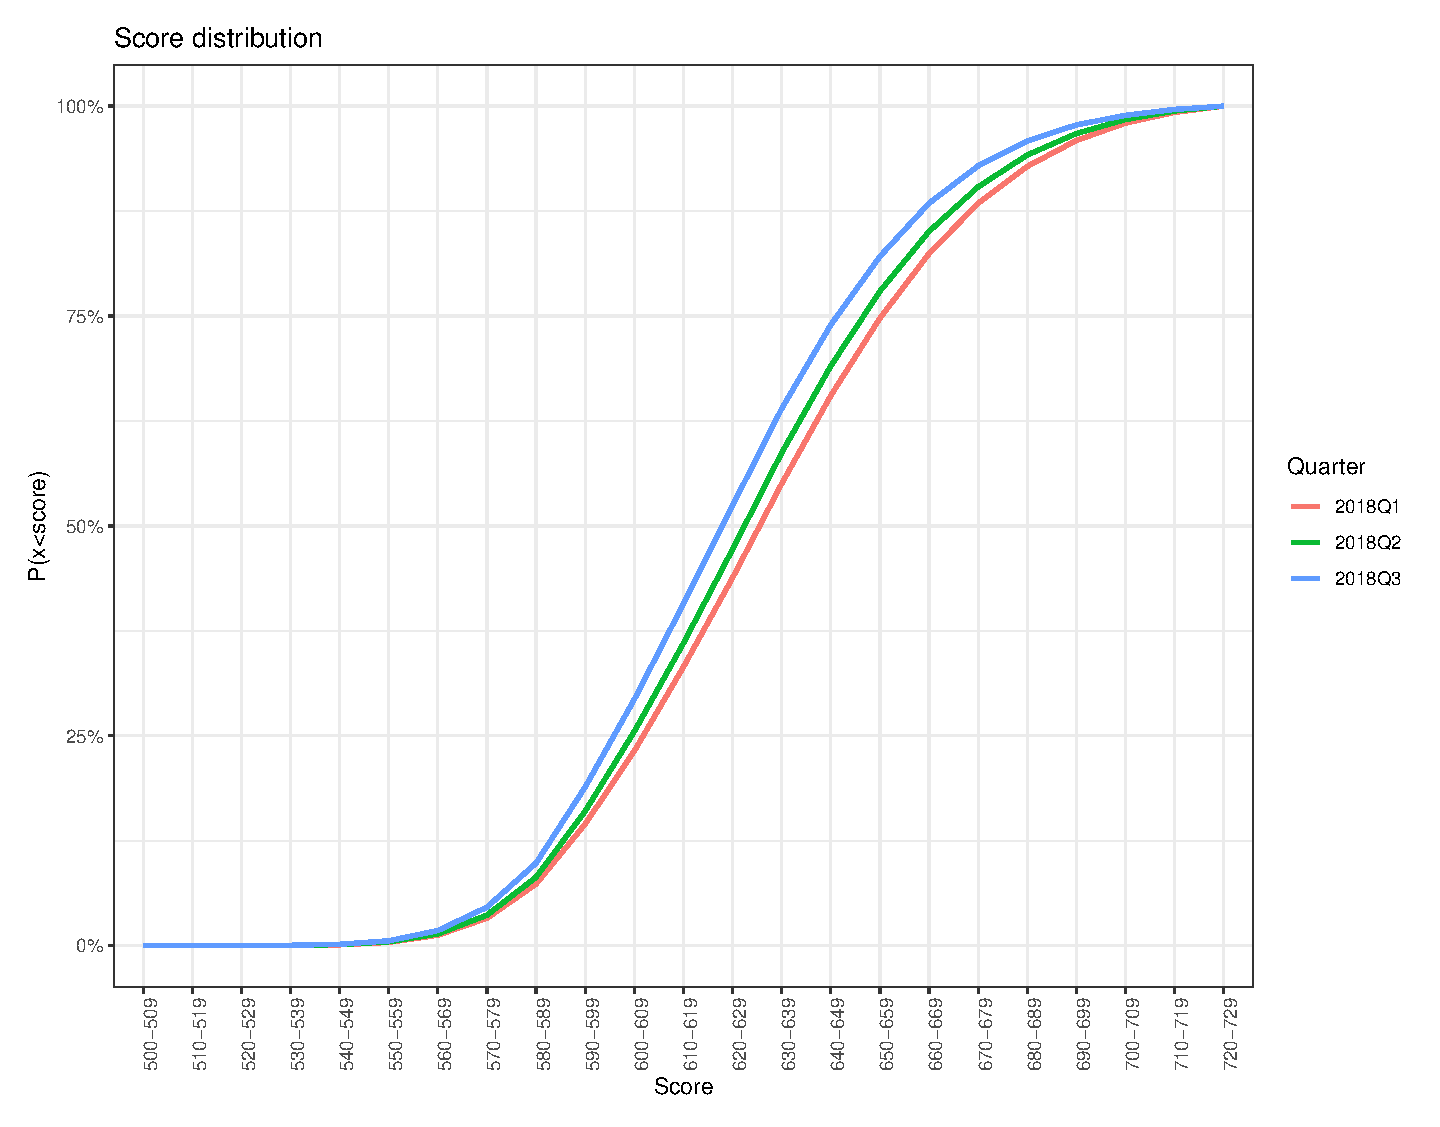
\includegraphics[width=5in,trim={0 0 0 0},clip]{content/figures/score_dev_nl.eps} 
  \caption{Score distribution each quarter of 2018. It is present that the score distribution is successively skewed to the left each quarter, this implies that the population is entailing higher risk and is a driver of the increase.}
  \label{fig:score_dev_1}
\end{figure}

\begin{figure}[!ht]
  \centering
  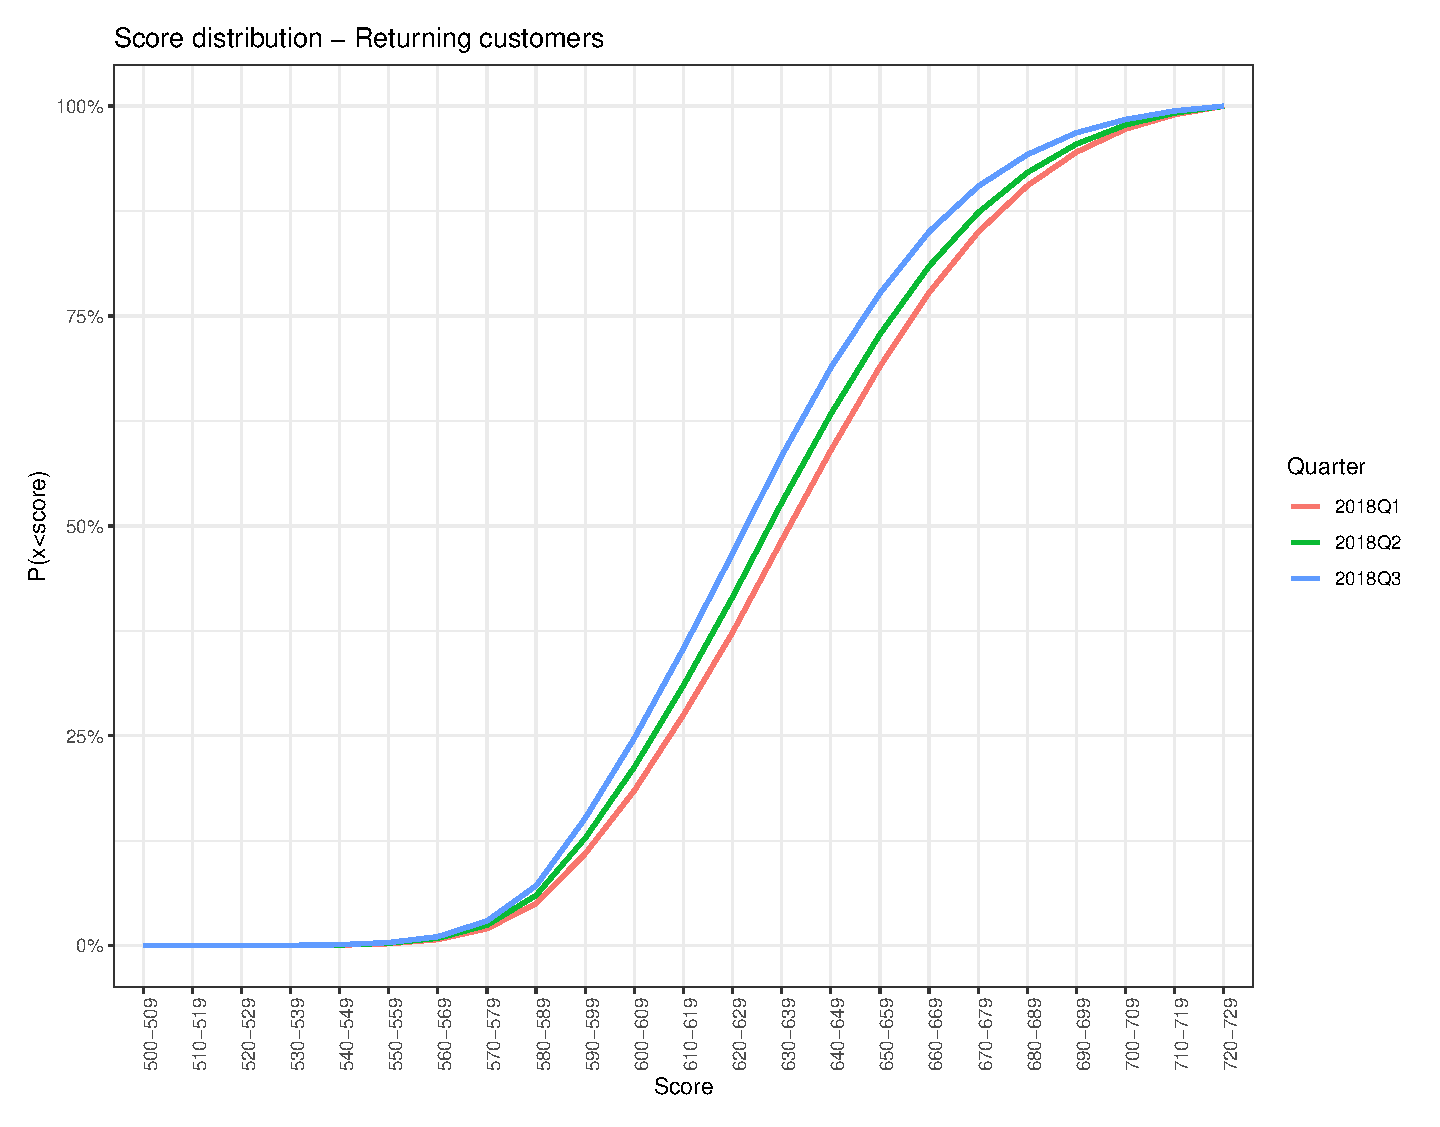
\includegraphics[width=5in,trim={0 0 0 0},clip]{content/figures/score_dev_nl_ret.eps} 
  \caption{Score distribution each quarter of 2018 for returning customers. The score distribution for returning customers shows the largest change during the period. It is evident that the distribution is significantly different fore each quarter.}
  \label{fig:score_dev_ret}
\end{figure}

\begin{figure}[!ht]
  \centering
  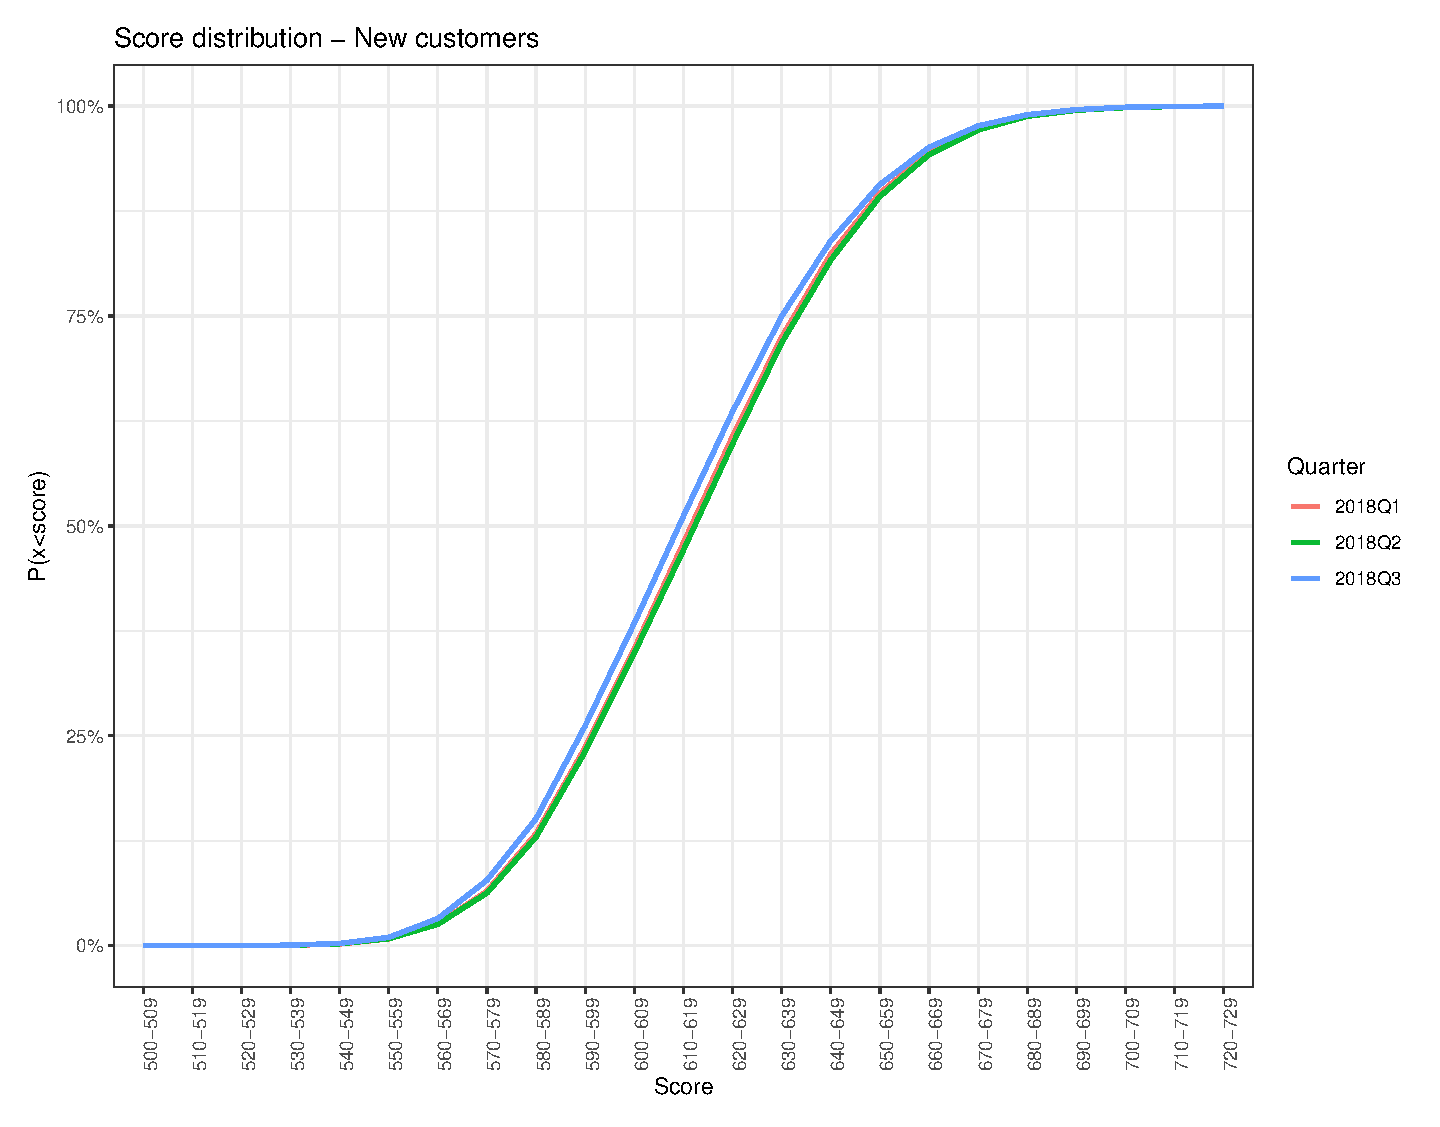
\includegraphics[width=5in,trim={0 0 0 0},clip]{content/figures/score_dev_nl_new.eps} 
  \caption{Score distribution each quarter of 2018 for new customers. It seems to be the case that the score distribution for new customers have changed just a little during the period.}
  \label{fig:score_dev_new}
\end{figure}

% -------------------------------------------------------------------------
% NEW VS. RETURNING CUSTOMERS
% -------------------------------------------------------------------------

\begin{figure}[!ht]
  \centering
  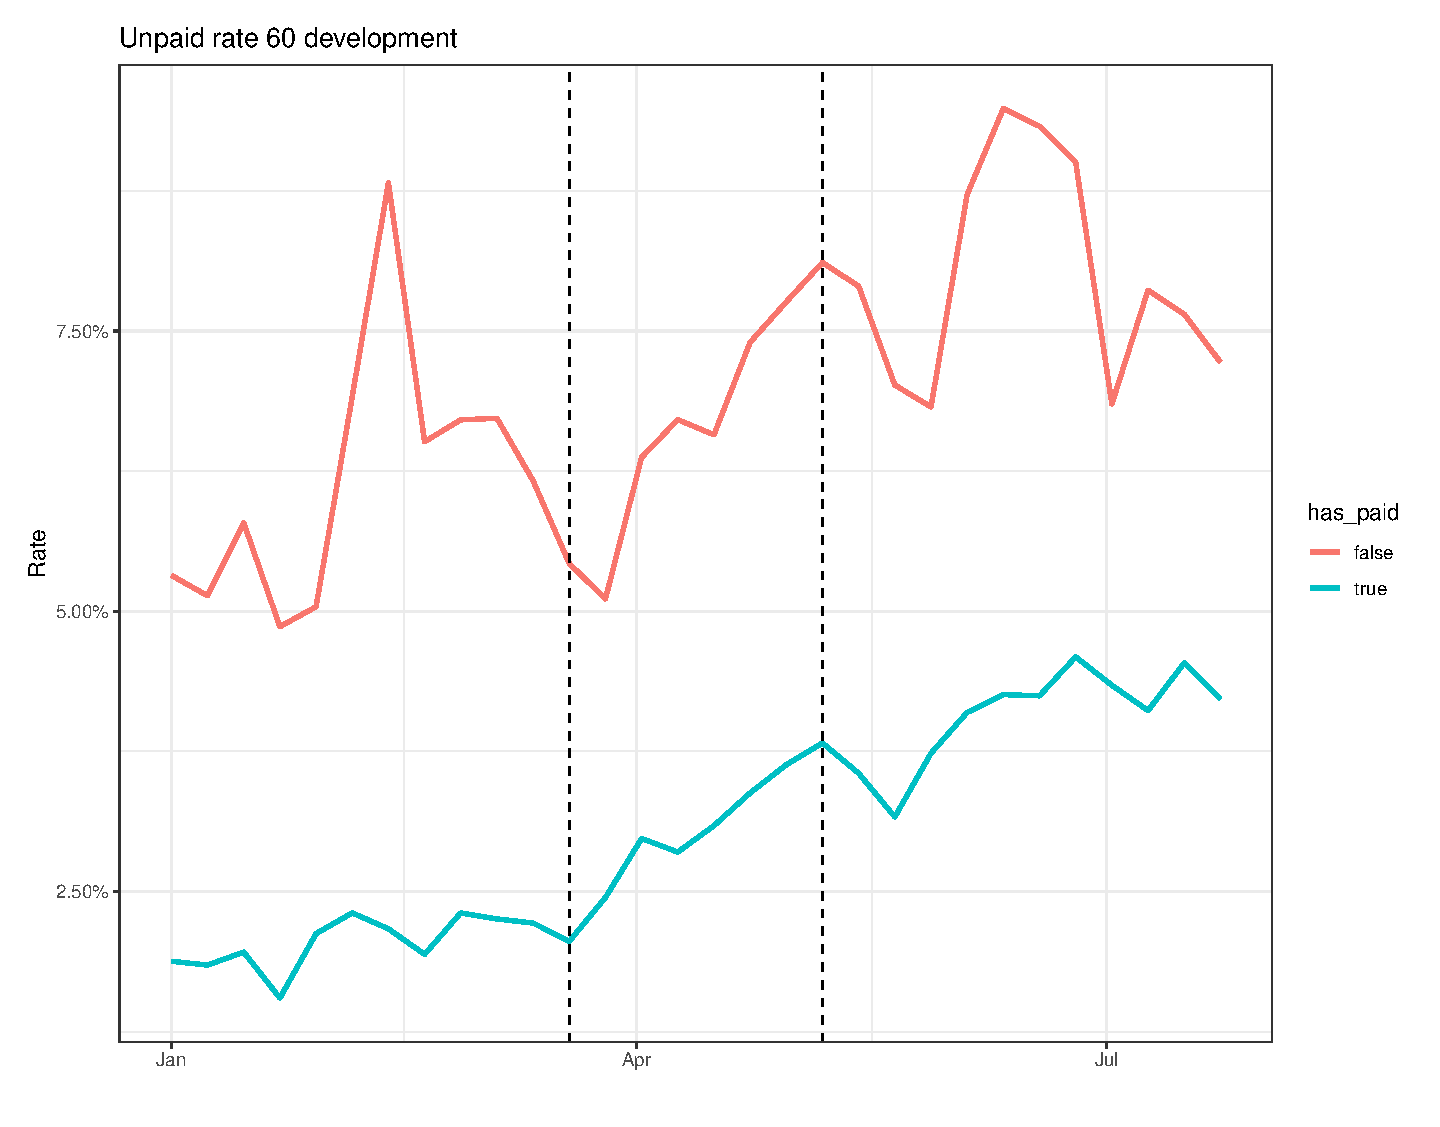
\includegraphics[width=5in,trim={0 0 0 0},clip]{content/figures/rate60_dev_nl_hp.eps} 
  \caption{Unpaid rate 60 for new and returning customers.}
  \label{fig:rate60_dev_hp}
\end{figure}

% -------------------------------------------------------------------------
% Different AOV intervals
% -------------------------------------------------------------------------

\begin{figure}[!ht]
  \centering
  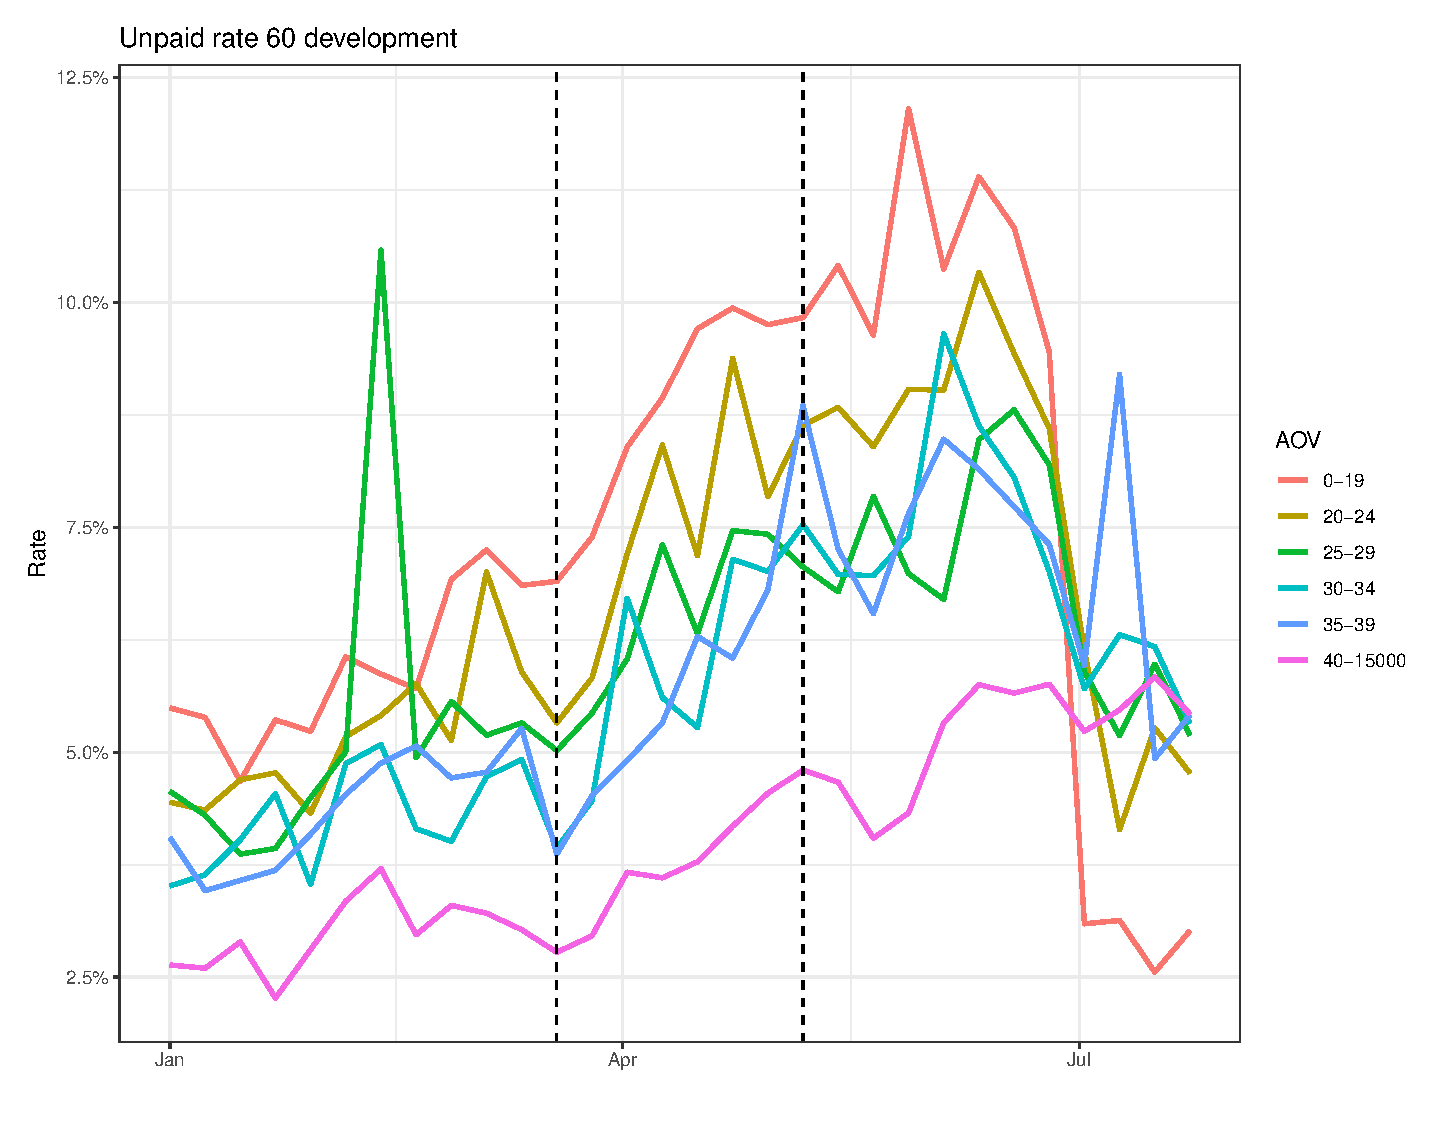
\includegraphics[width=5in,trim={0 0 0 0},clip]{content/figures/rate60_dev_nl_aovbin.eps} 
  \caption{Unpaid rate 60 for different AOV bins.}
  \label{fig:rate60_dev_aov}
\end{figure}

\begin{figure}[!ht]
  \centering
  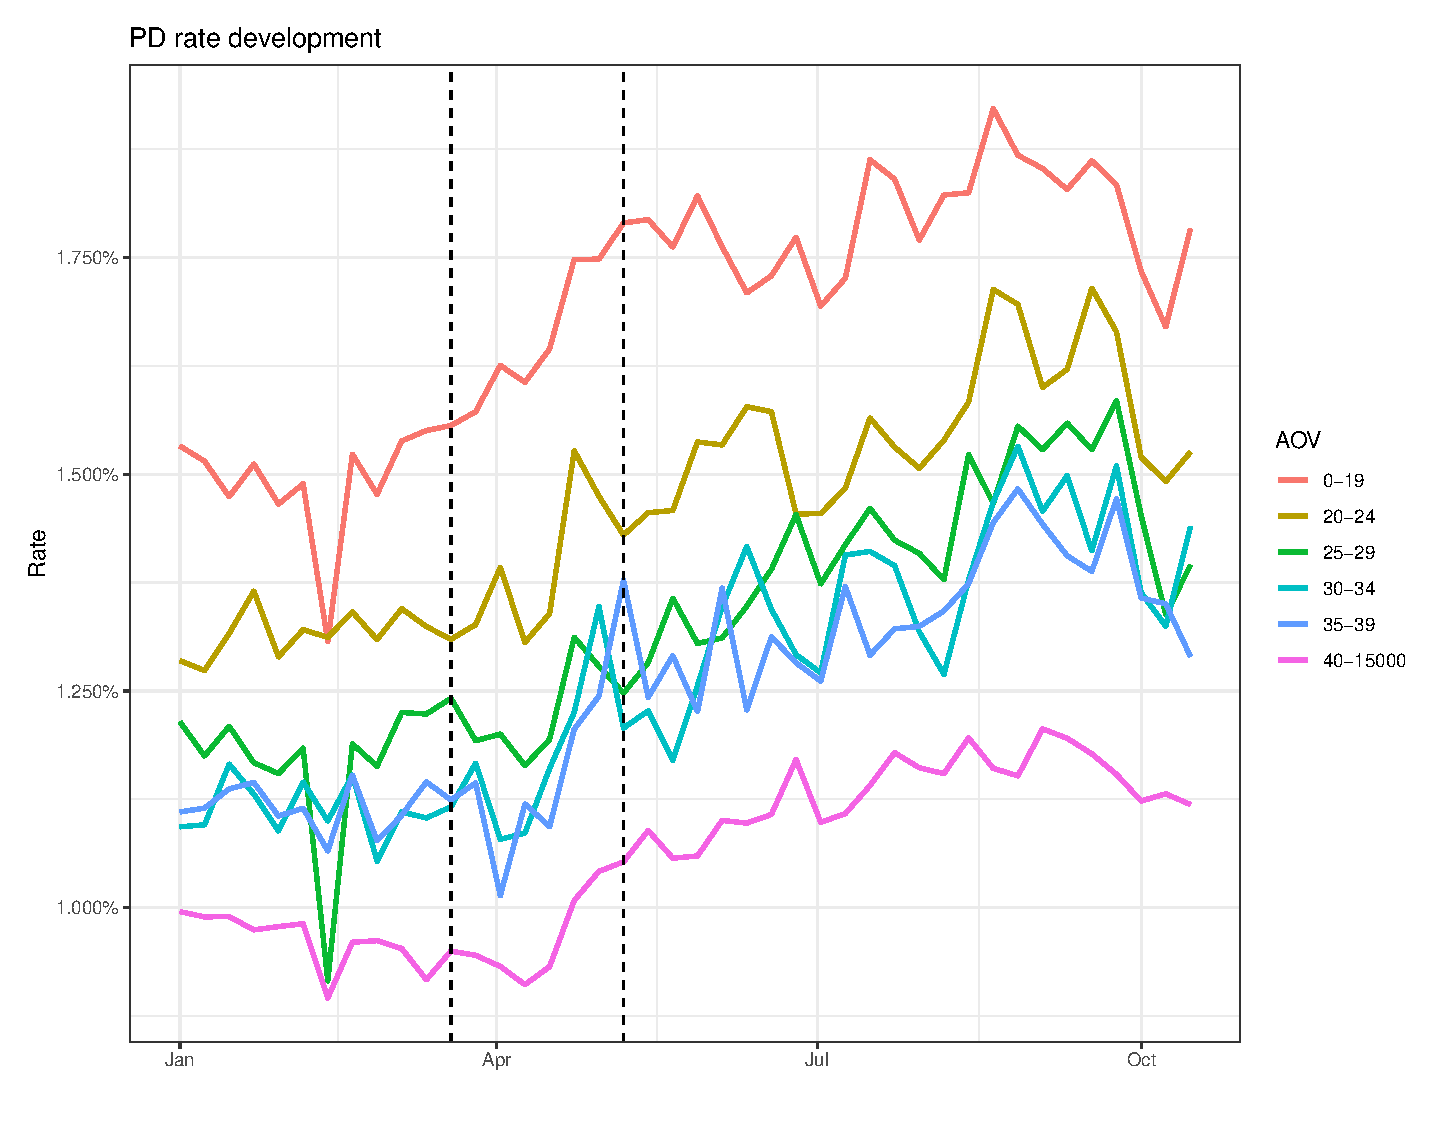
\includegraphics[width=5in,trim={0 0 0 0},clip]{content/figures/pd_dev_nl_aovbin.eps} 
  \caption{PD rate for different AOV bins.}
  \label{fig:pd_dev_aov}
\end{figure}


% -------------------------------------------------------------------------
% Unpaid 90 vs. PD
% -------------------------------------------------------------------------

\begin{figure}[!ht]
  \centering
  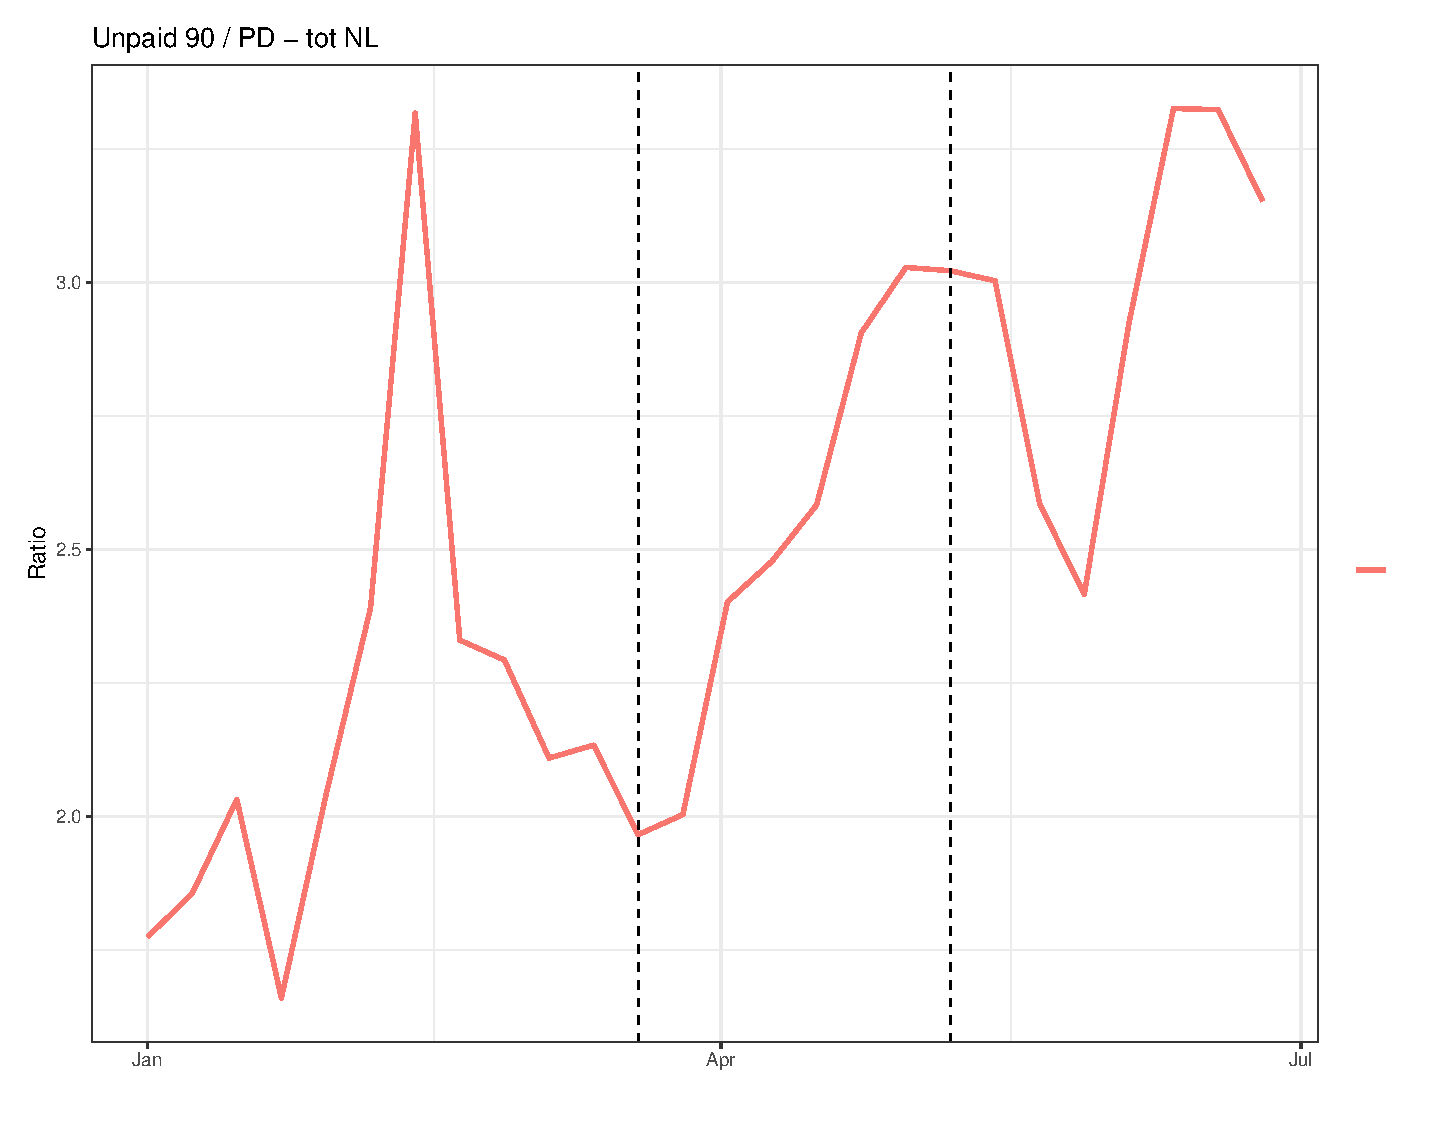
\includegraphics[width=5in,trim={0 0 0 0},clip]{content/figures/unp90pd_dev_nl.eps} 
  \caption{Unpaid rate 90 vs. PD rate. The ratio is increasing during the period. Since we know that PD is increasing the conclusion is that unpaid rate 90 is increasing at a faster rate than the PD rate. This is not surprising since from looking into the score development we saw that PD is growing but it did not explain the total increase.}
  \label{fig:unp90pd_dev}
\end{figure}

\begin{figure}[!ht]
  \centering
  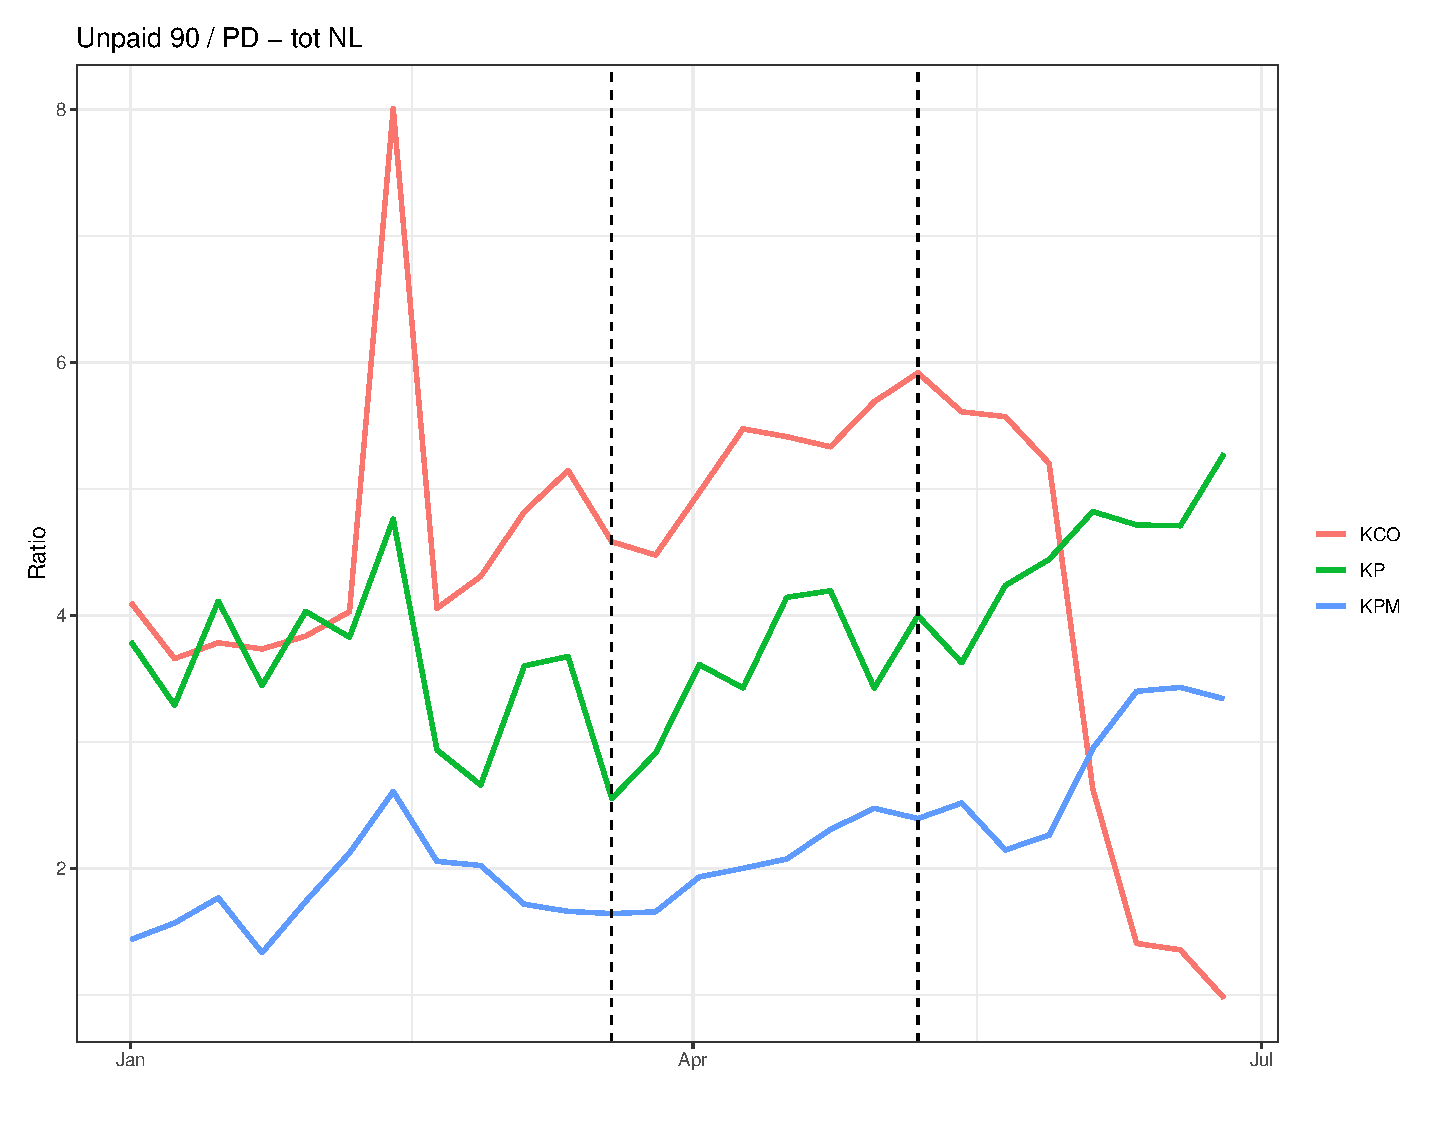
\includegraphics[width=5in,trim={0 0 0 0},clip]{content/figures/unp90pd_dev_nl_as.eps} 
  \caption{Unpaid rate 90 vs. PD rate for the different acquiring sources.}
  \label{fig:unp90pd_dev_as}
\end{figure}


% -------------------------------------------------------------------------
% Scorecard to use
% -------------------------------------------------------------------------

\begin{figure}[!ht]
  \centering
  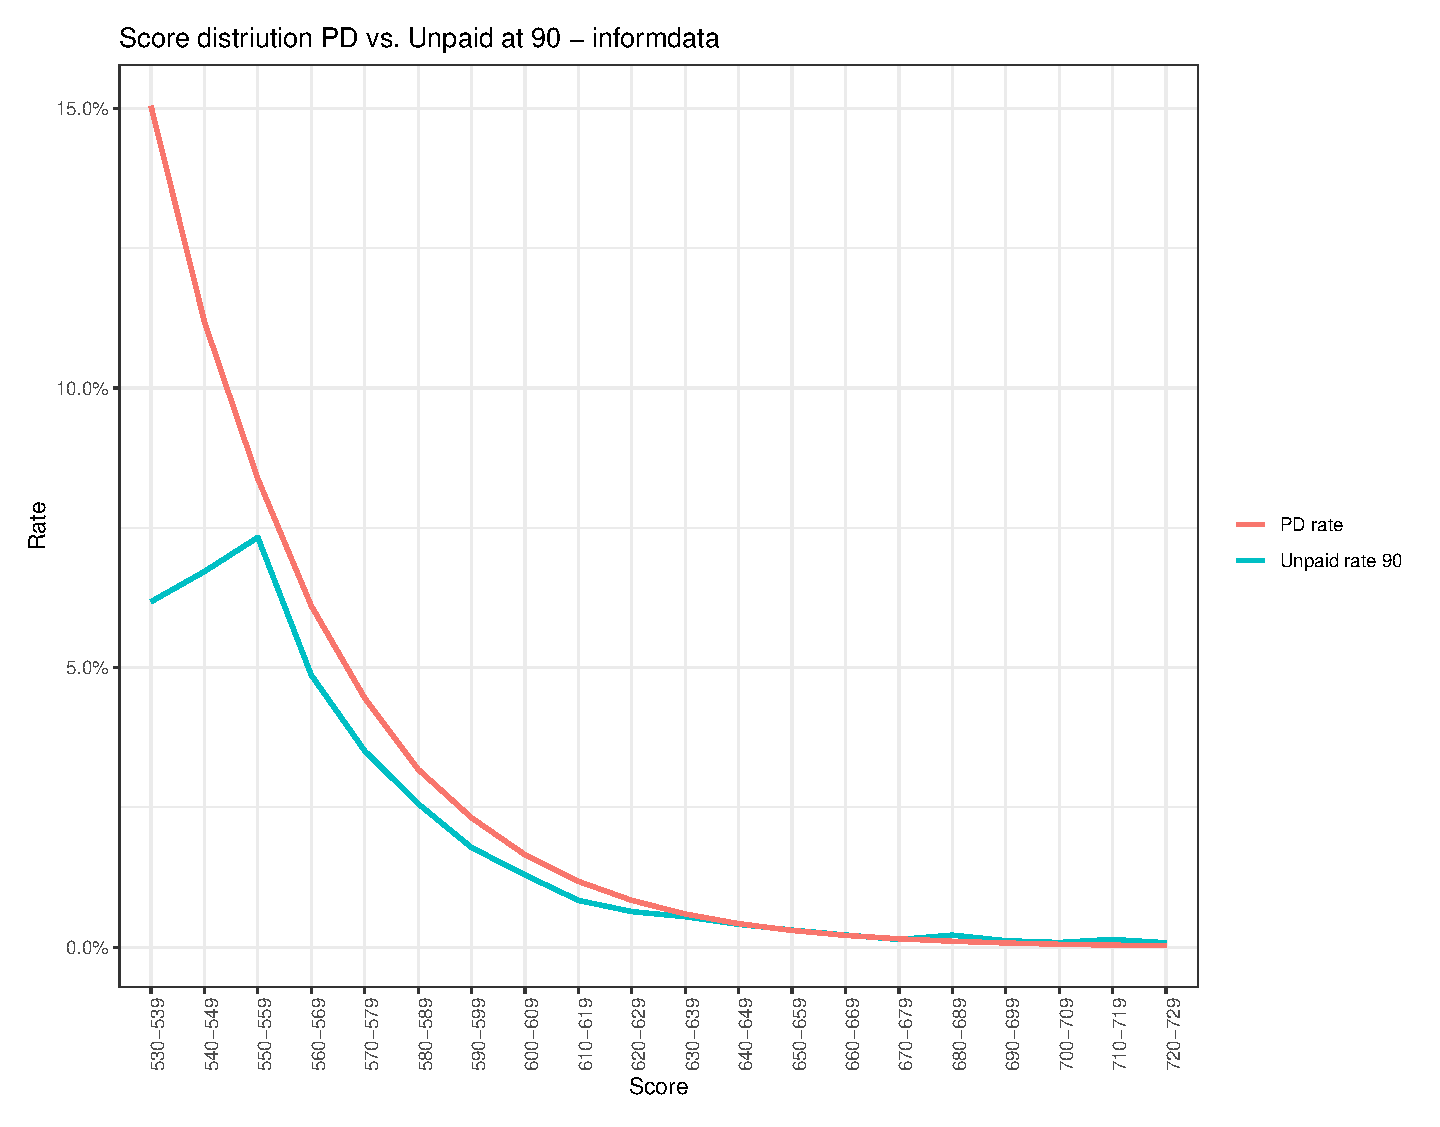
\includegraphics[width=5in,trim={0 0 0 0},clip]{content/figures/scdist_dev_informdata.eps} 
  \caption{PD rate vs. unpaid at 90 rate for scorecard informdata. Largest scorecard.}
  \label{fig:scdist_dev_informdata}
\end{figure}

\begin{figure}[!ht]
  \centering
  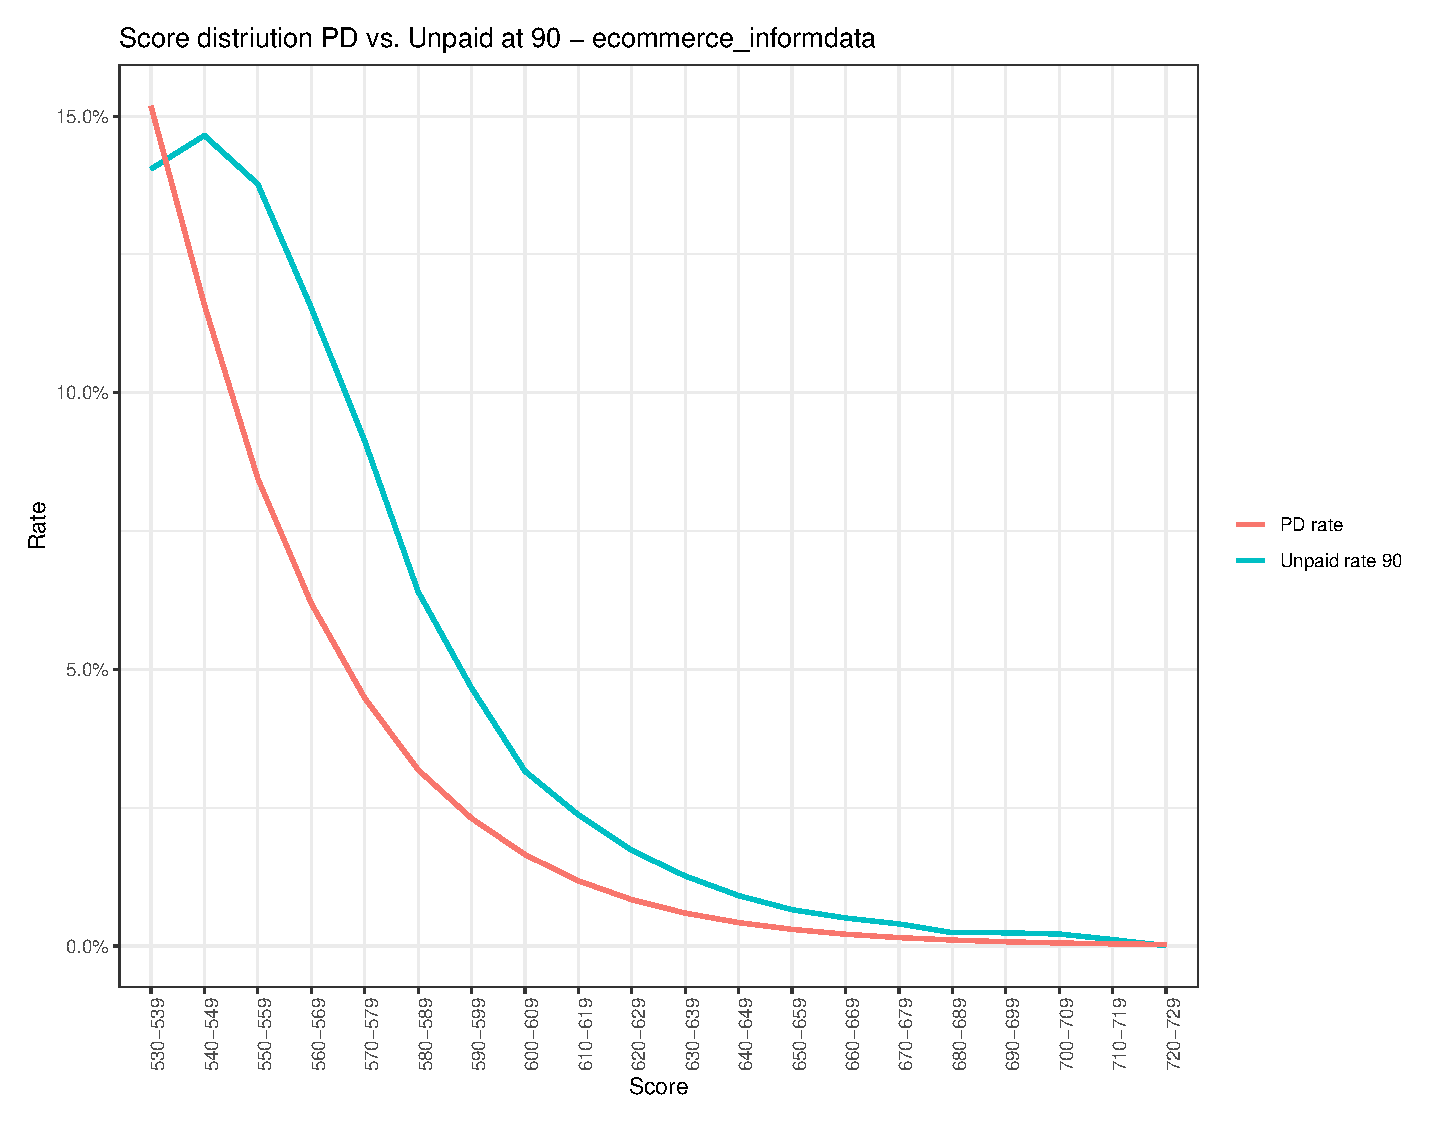
\includegraphics[width=5in,trim={0 0 0 0},clip]{content/figures/scdist_dev_ecommerce_informdata.eps} 
  \caption{PD rate vs. unpaid at 90 rate for scorecard ecomerce\_informdata. Second largest scorecard.}
  \label{fig:scdist_dev_ecommerce_informdata}
\end{figure}































